\part{Conception d'ensemble}
\setcounter{section}{0}

\section{Modèles conceptuels de données} 

\subsection{Données clients et produits} 

\begin{figure}[H]
\centering
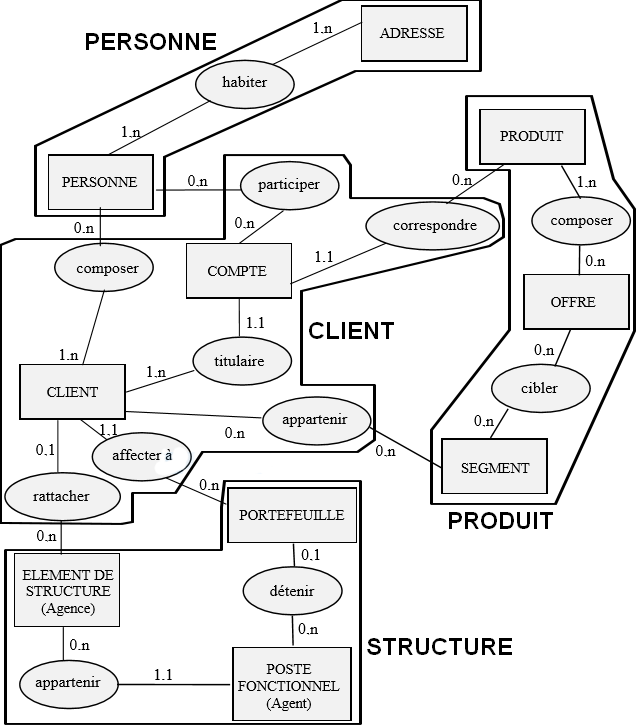
\includegraphics[width=\textwidth]{figures/mcd/MCD_Clients_Produits}
\caption{MCD Clients Produits}
\end{figure}


\subsection{Données commerciales}

\begin{figure}[H]
\centering
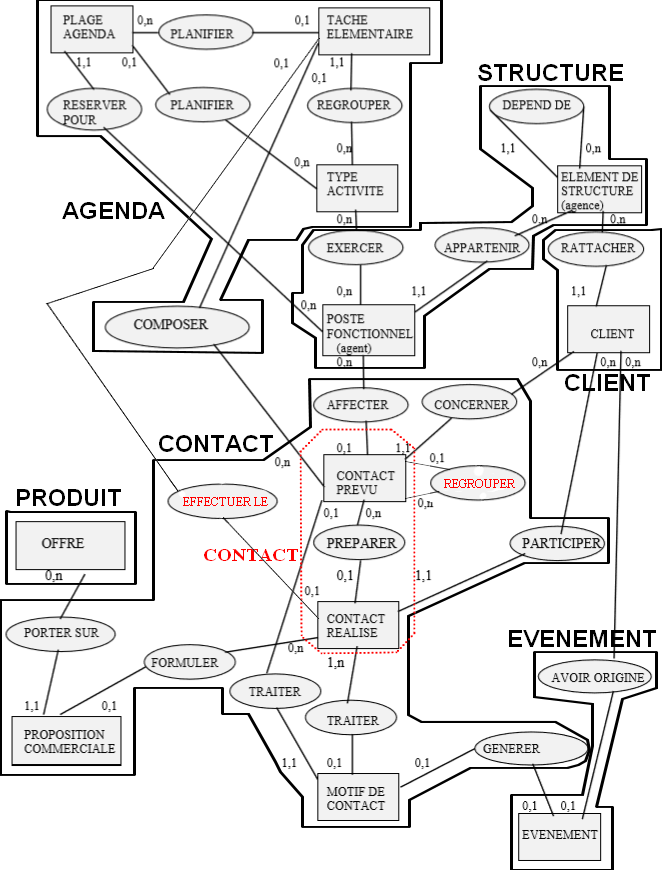
\includegraphics[width=\textwidth]{figures/mcd/MCD_Commercial}
\caption{MCD Commercial}
\end{figure}

\section{Diagramme d’état de l'objet métier \bf{contact}}

\begin{figure}[H]
\centering
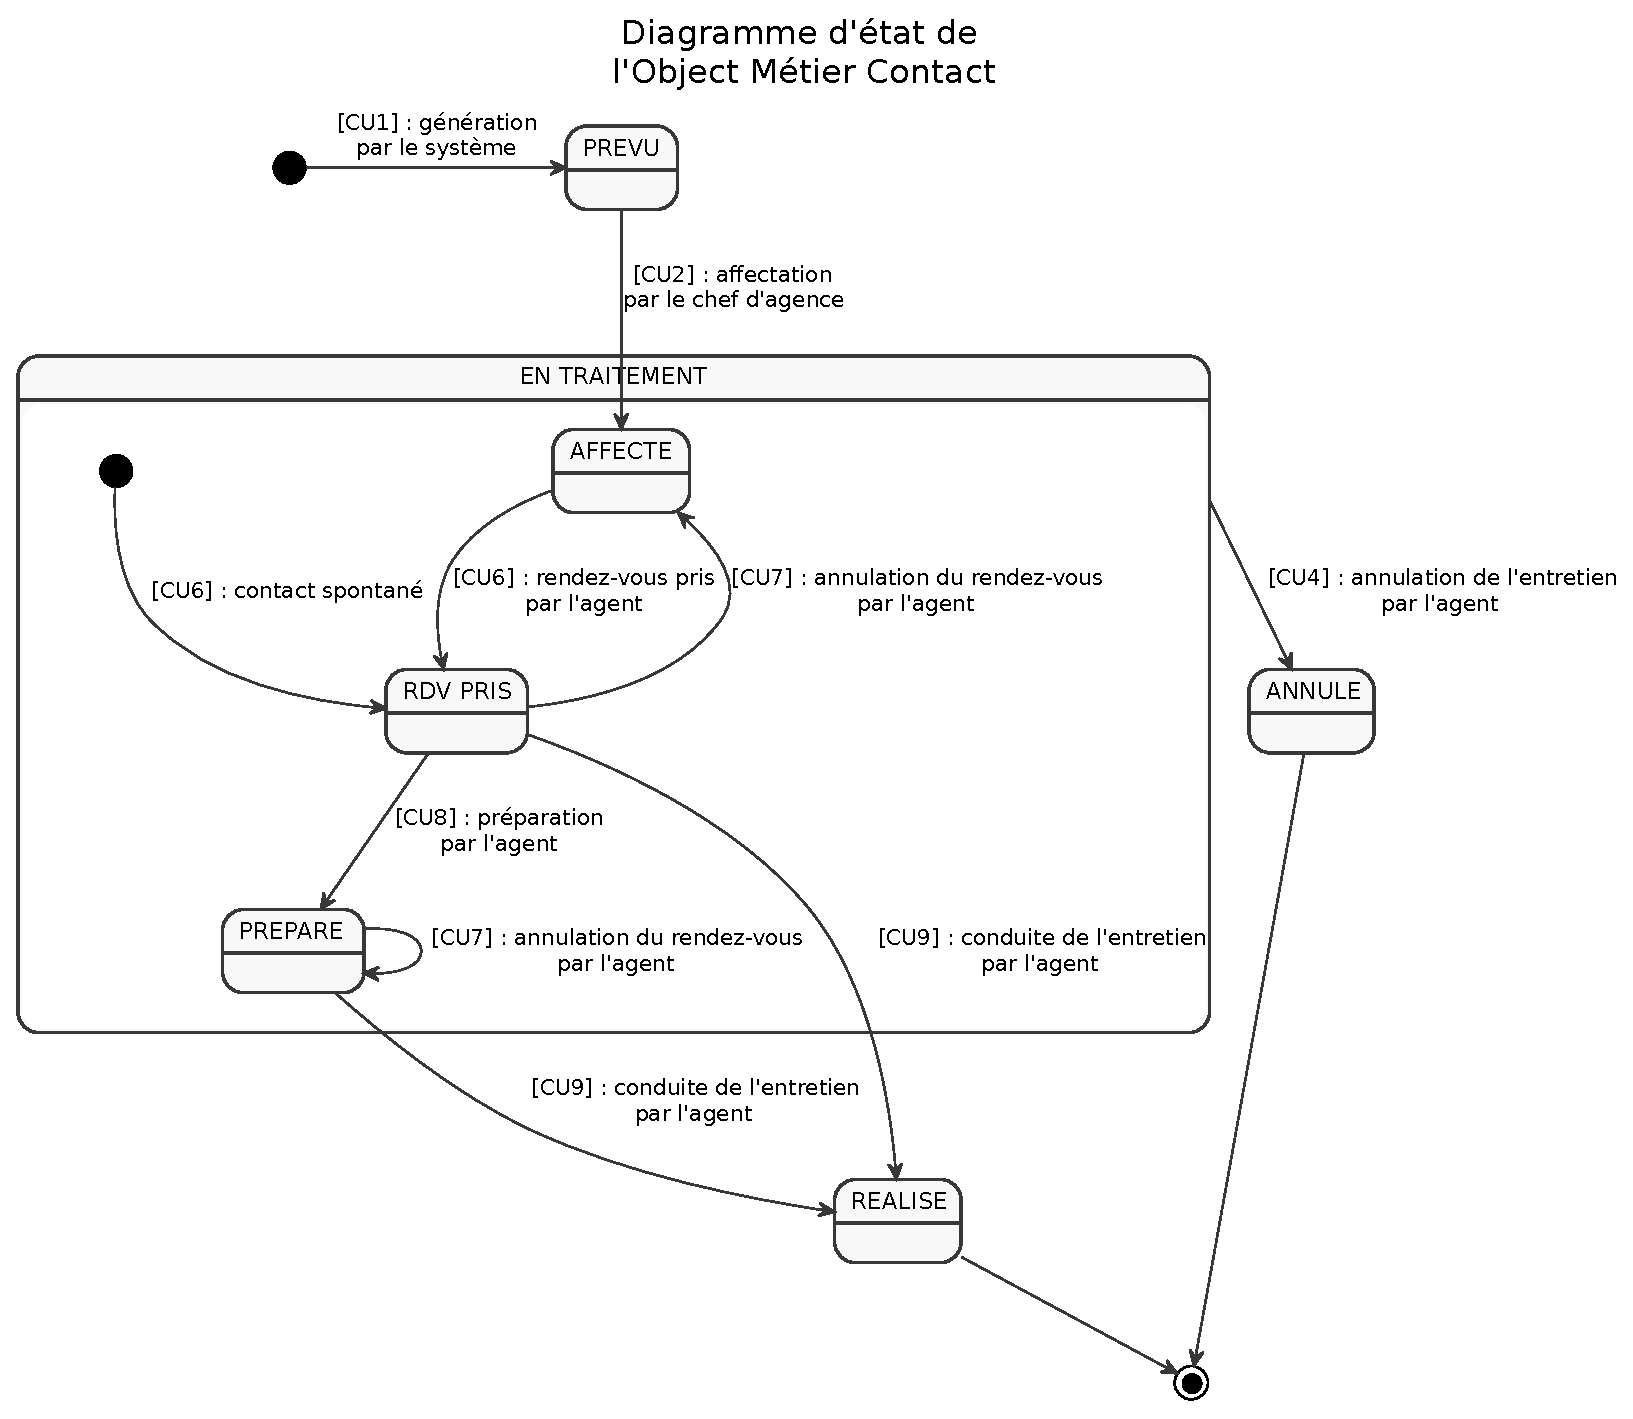
\includegraphics[width=\textwidth]{figures/eps/diag_etats_contact}
\caption{Diagramme d'état de l'objet métier contact}
\end{figure}

\section{Choix  de  l’environnement  technique}
L’environnement  technique  déjà  retenu  par  la 
Maîtrise d’Ouvrage (MOA) de la banque est une architecture C/S n-tiers. 